\chapter{Radio packet format and retransmission scheme}\label{chap4}

The sensors communicate with a base station with a unidirectional radio link. There is no receiver module in the sensors. They can not have any kind of acknowledgement of their transmission, nor can they do carrier detection. The system has no means to verify whether a packet has been delivered successfully. Therefore, we design a retransmission scheme in order to improve event deliver rate. 

\section{Radio packet format and retransmission scheme}

In our design, each packet has 16-bit of payload plus one parity bit. Each packet is 64 milliseconds long, which is slightly less than 4 AC cycles (assuming 60Hz). Hence, we choose 4 AC cycles as a time slot for transmission. 

When a sensor detects an event, it transmits 5 packets in a timespan of 2.2 seconds. The event is successfully delivered when at least one packet is successfully received. In the rare case that another event detected on the same sensor before it finishes with the previous event, any further retransmissions of the previous event are cancelled. We call the previous event a \textit{flash event}. 

The sensor can detect zero-crossing of AC voltage, and use that to provide a 60Hz timer synchronous to AC cycles. All packet transmissions are synchronized to AC cycles. 

\begin{figure}[htb]
  \centering
  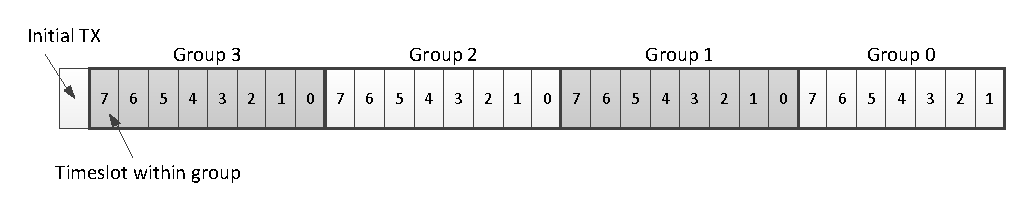
\includegraphics[width=\textwidth]{figures/slots}
  \caption[Transmission timeslots]{Transmission timeslots: There is an initial transmission, followed by 4 groups of timeslots. One slot is randomly picked from each group for a retransmission. }
  \label{fig:slots}
\end{figure}

When an event is detected, the sensor initiated a transmission at the next AC cycle. Following the initial time slot, there are 31 more slots, arranged in 4 groups. The groups have 8, 8, 8 and 7 time slots respectively. Fig.\ref{fig:slots} shows the arrangement of transmission time slots. The sensor randomly pick one slot from each group. Altogether there are 32 time slots, or 128 cycles, roughly 2.2 seconds. 

\begin{figure}[htb]
  \centering
  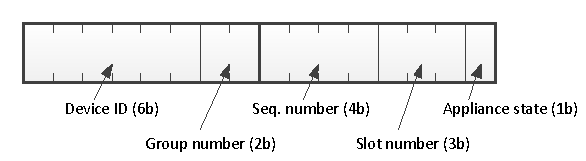
\includegraphics[width=0.8\textwidth]{figures/packet}
  \caption{16-bit packet format}
  \label{fig:packet}
\end{figure}

The format of each packet is shown in Fig.\ref{fig:packet}. The initial transmission of an event will have group number 0 and slot number 0. The group and slot number are included in the packet so that the receiver can estimate the delay from the event to the transmission. The 4-bit sequence number is advanced in every packet. The 6-bit device ID is hardcoded in every sensor node, allowing up to 64 sensors working in a same region with a single receiver. 

\section{Evaluation of the radio network}

The evaluation of our sensor network is presented in three parts: simulations, a controlled testbed, and a real setting. 

We have two abbreviations used throughout this section: $PDR$ and $EDR$. Packet delivery ratio ($PDR$) is the ratio of successfully received packets among all transmitted packets. Event delivery ratio ($EDR$) is the ratio of successfully delivered events among all detected events. Because of the redundancy of packets, an event loss happens only when all packets of the event are lost. 

%In simulation, we assume guaranteed delivery of packets as long as packets are not corrupted because of collision. In a controlled setup, we use an extra microcontroller to generate events, and the sensor nodes are placed close to the receiver. In the real setting, we deployed 20 sensors in our lab. The deployment will be discussed in detail in Chapter \ref{chap5}.

\subsection{Simulation: Poisson distribution events}

We develop a simulator according to our packet format and retransmission scheme. The simulator is capable to simulate at packet level in the continuous time domain. It detects packet collisions, which guarantee packet loss, and mimics a constant $PDR_0$ due to reasons other than collisions. Note that because of collision, the overall $PDR$ is guaranteed to be less than or (in case of no collision) equal to $PDR_0$. $PDR_0$ represents the power delivery ratio inherent to the sensor itself such as transmitter power, or deployment such as distance to the receiver. 

The test datasets are synthesized according to the following assumptions. 1) Appliances are independent with each other; 2) Events on appliance $A_k$ conform to a poisson distribution with parameter $\lambda_k$; 3) All appliances have the same poisson distribution parameter, i.e. $\lambda_k = \lambda$ for all $k$. Here $\lambda$ is the average number of events happend in 1 second on a single appliance. And $\mu = 1/\lambda$ is the expected interval between two events of an appliance. 

According to these assumptions, the overall events of all appliances conform to a poisson distribution with parameter $N\lambda$, where $N$ is the number of appliances. In another word, the density of events can be adjusted ether by adjusting $N$ or adjusting $\lambda$, ignoring flash events. Taking flash events into account, the result of high $N$ and high $\lambda$ are not exactly the same. In the case of high $\lambda$, there are more flash events, and they are more vulnerable to loss because they do not have all 5 transmission. In the case of high $N$, there are more chances of collision. 

In this simulation, we synthesize the datasets with a fixed $N=6$, and let $\mu$ vary from 3 to 20, which means the expected interval between events of an appliance is 3 to 20 seconds. Note that here $\mu$ is much shorter than what we would expect in real settings. In real settings, appliances do not frequently change state in tens of seconds. We choose the numbers on purpose to stress our network. Each dataset consists of 1500 events in total, 250 from each sensor. 

Firstly, we evaluate the effect of having multiple retransmissions for each event. We assume all sensors have the same $PDR_0$. And sensors are independent with each other. Fig.\ref{fig:retrans-lambda-0.4}-\ref{fig:retrans-lambda-1} shows the effect of multiple retransmissions on $EDR$ and $PDR$ under different $\mu$, with several fixed values of $PDR_0$. 

\begin{figure}[p]
    \centering
    \begin{subfigure}[t]{0.9\textwidth}
        \centering
        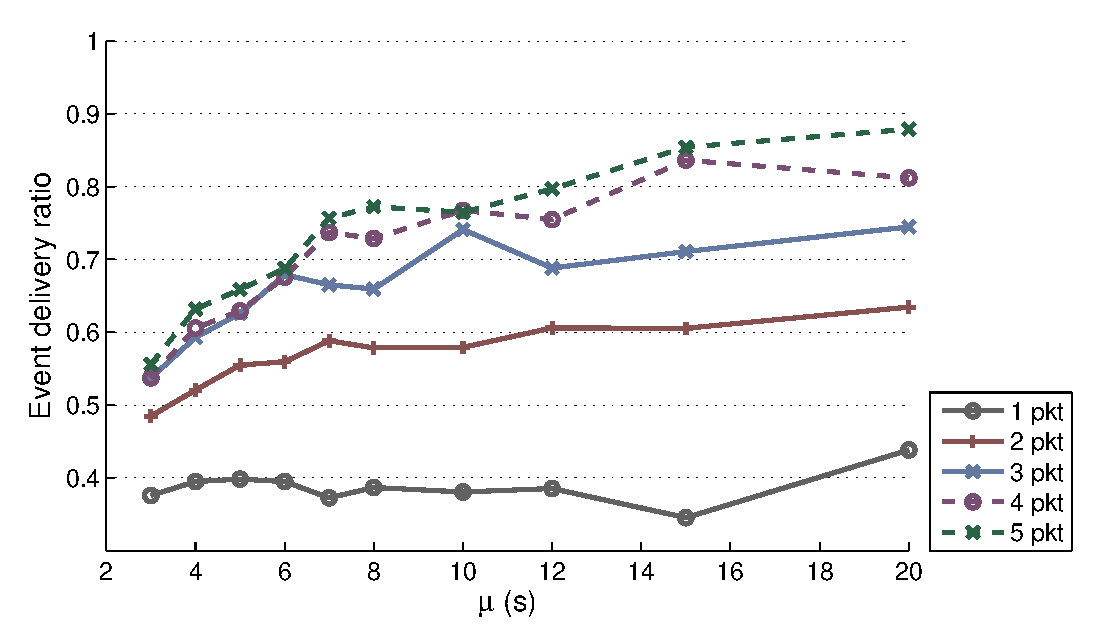
\includegraphics[width=\textwidth] {../../sw/pc/matlab/simulation-result/retrans-count-edr-20min-pdr0.4.eps}
        \caption{}
    \end{subfigure} 
    \\
    \begin{subfigure}[t]{0.9\textwidth}
        \centering
        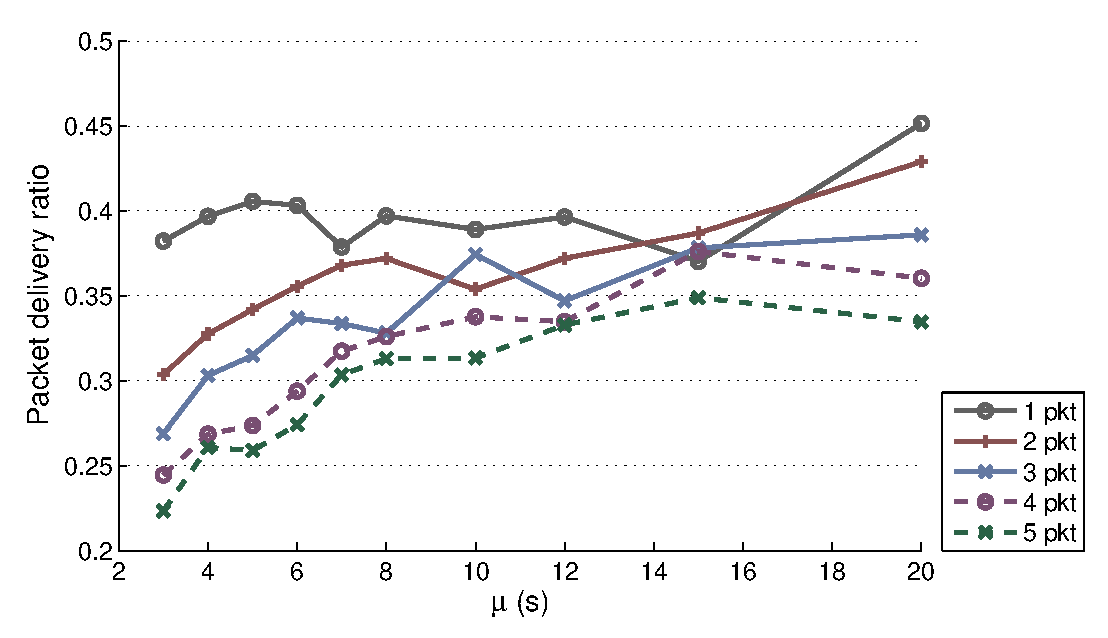
\includegraphics[width=\textwidth] {../../sw/pc/matlab/simulation-result/retrans-count-pdr-20min-pdr0.4.eps}
        \caption{}
    \end{subfigure}
    \caption[EDR and PDR with different transmission redundancy, $PDR_0 = 0.4$]{Simulation results showing EDR(a) and PDR(b) with different number of retransmissions per event, at $PDR_0 = 0.4$}\label{fig:retrans-lambda-0.4}
\end{figure}


\begin{figure}[p]
    \centering
    \begin{subfigure}[t]{0.9\textwidth}
        \centering
        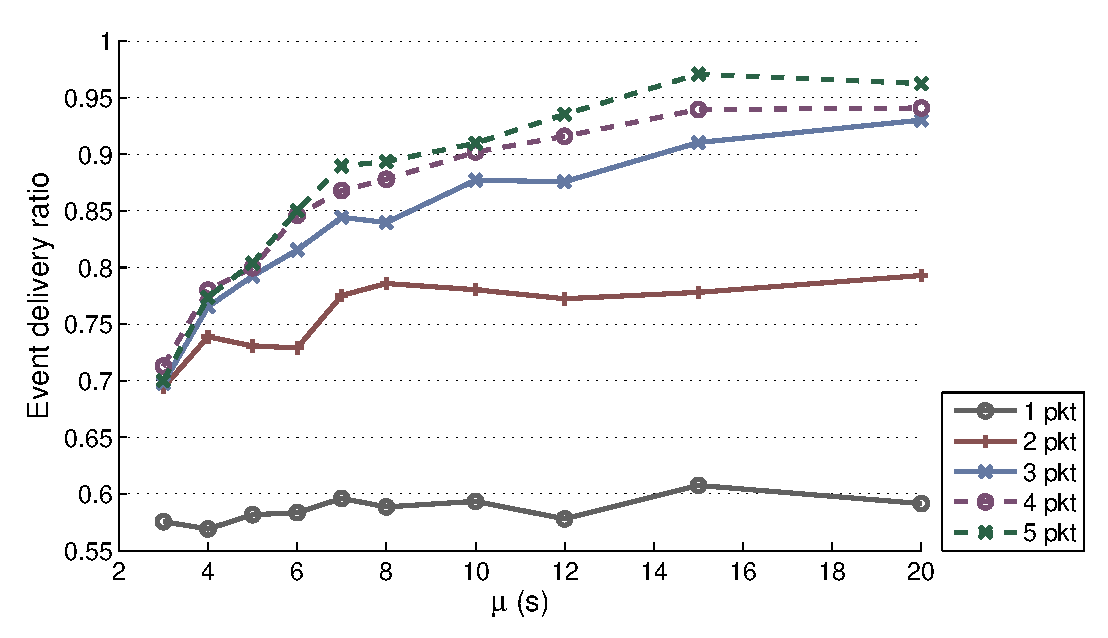
\includegraphics[width=\textwidth] {../../sw/pc/matlab/simulation-result/retrans-count-edr-20min-pdr0.6.eps}
        \caption{}
    \end{subfigure} 
    \\
    \begin{subfigure}[t]{0.9\textwidth}
        \centering
        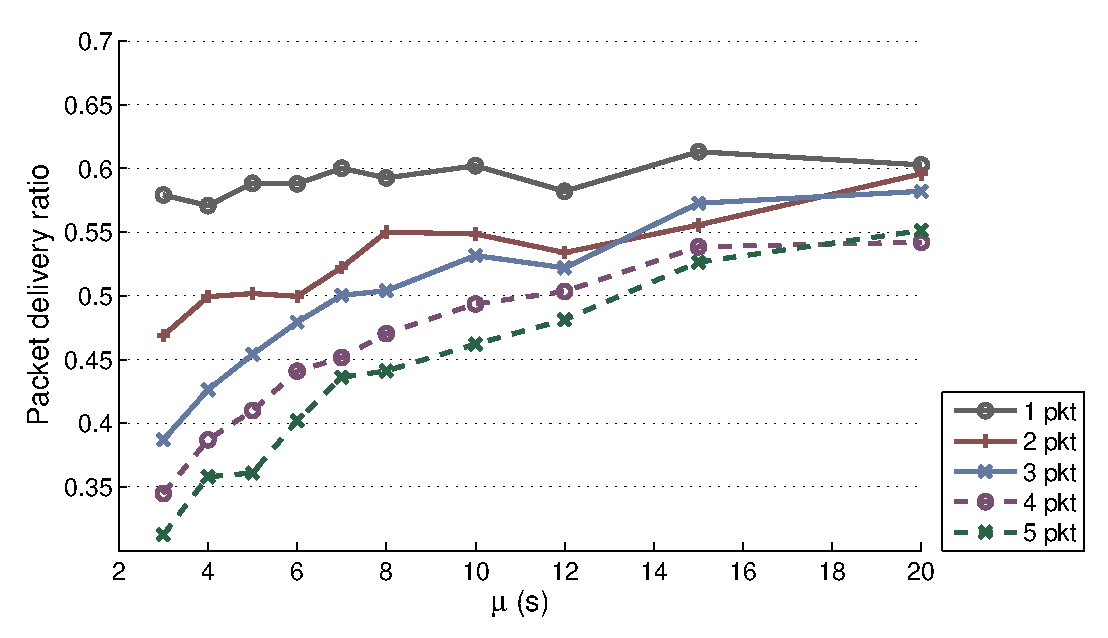
\includegraphics[width=\textwidth] {../../sw/pc/matlab/simulation-result/retrans-count-pdr-20min-pdr0.6.eps}
        \caption{}
    \end{subfigure}
    \caption[EDR and PDR with different transmission redundancy, $PDR_0 = 0.6$]{Simulation results showing EDR(a) and PDR(b) with different number of retransmissions per event, at $PDR_0 = 0.6$}\label{fig:retrans-lambda-0.6}
\end{figure}


\begin{figure}[p]
    \centering
    \begin{subfigure}[t]{0.9\textwidth}
        \centering
        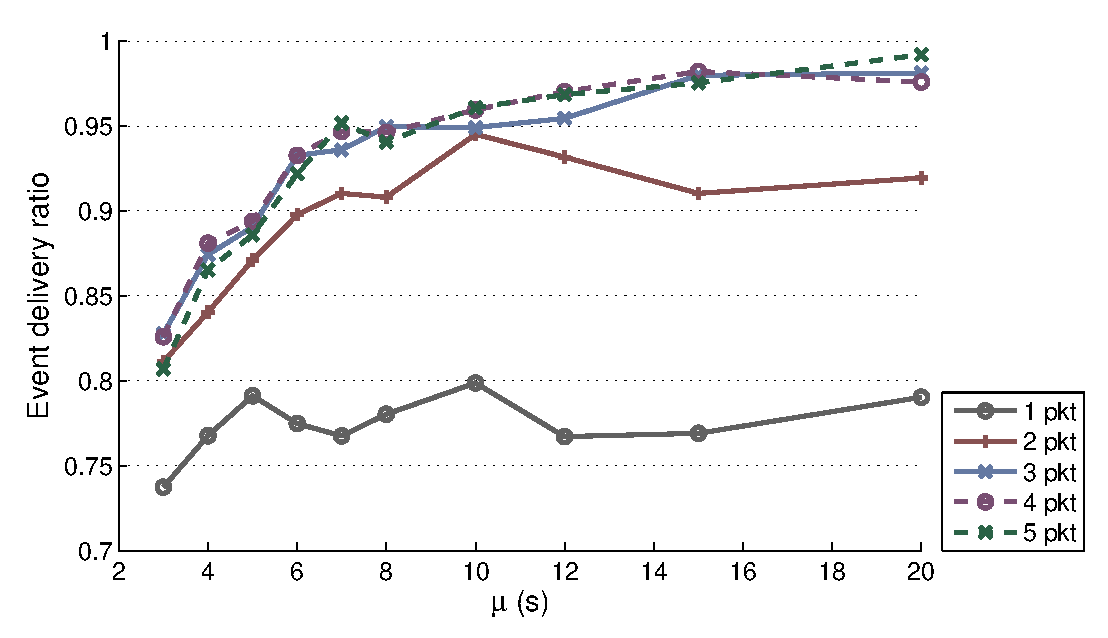
\includegraphics[width=\textwidth] {../../sw/pc/matlab/simulation-result/retrans-count-edr-20min-pdr0.8.eps}
        \caption{}
    \end{subfigure} 
    \\
    \begin{subfigure}[t]{0.9\textwidth}
        \centering
        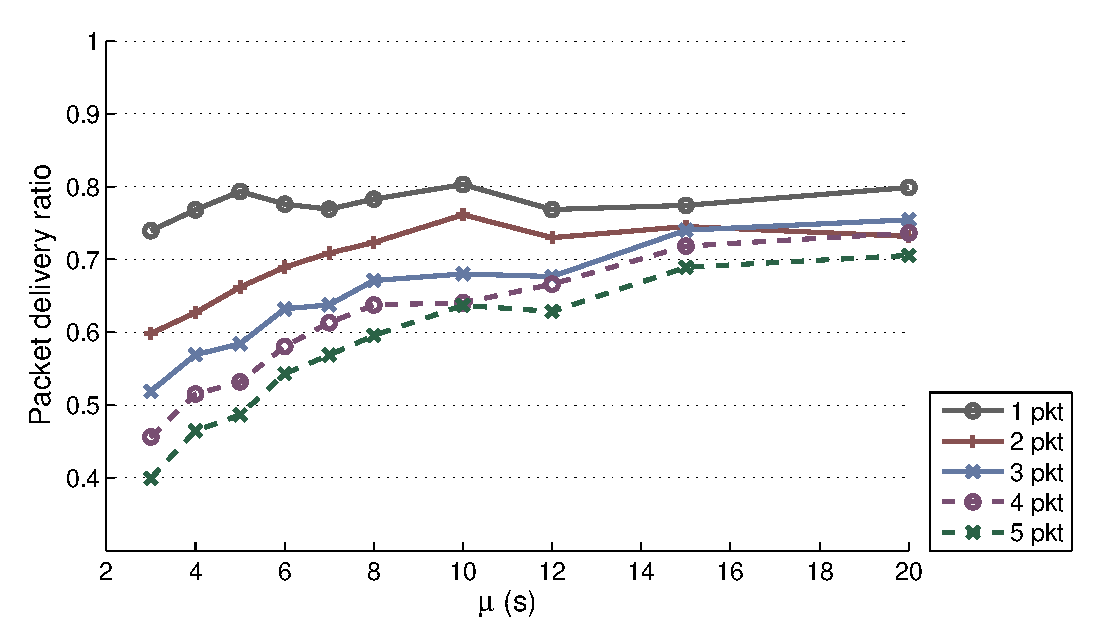
\includegraphics[width=\textwidth] {../../sw/pc/matlab/simulation-result/retrans-count-pdr-20min-pdr0.8.eps}
        \caption{}
    \end{subfigure}
    \caption[EDR and PDR with different transmission redundancy, $PDR_0 = 0.8$]{Simulation results showing EDR(a) and PDR(b) with different number of retransmissions per event, at $PDR_0 = 0.8$}\label{fig:retrans-lambda-0.8}
\end{figure}


\begin{figure}[p]
    \centering
    \begin{subfigure}[t]{0.9\textwidth}
        \centering
        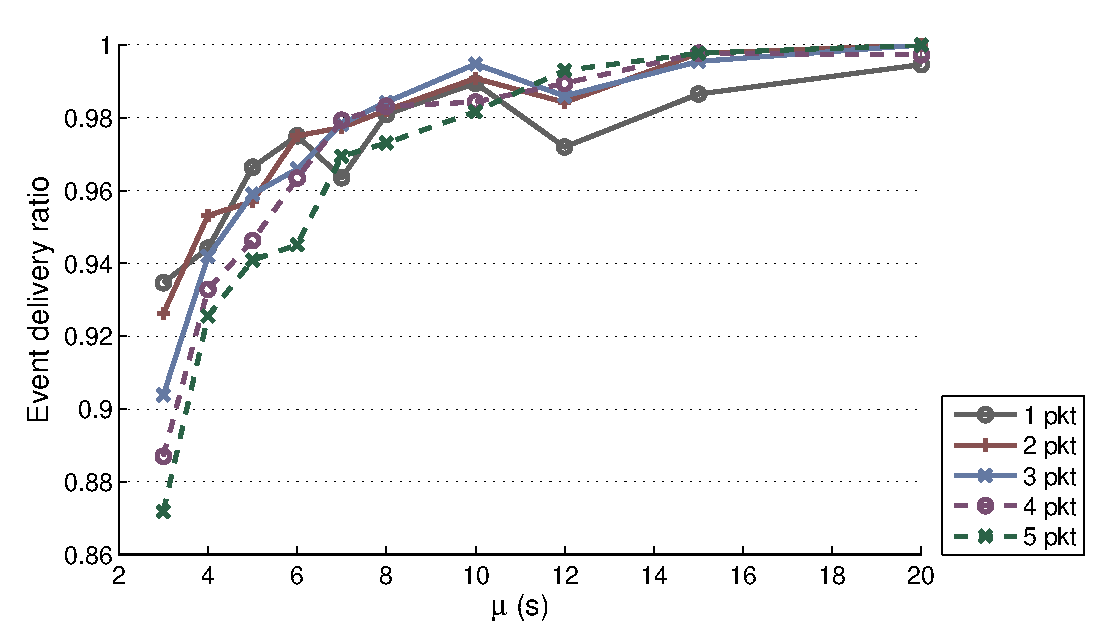
\includegraphics[width=\textwidth] {../../sw/pc/matlab/simulation-result/retrans-count-edr-20min-pdr1.eps}
        \caption{}
    \end{subfigure} 
    \\
    \begin{subfigure}[t]{0.9\textwidth}
        \centering
        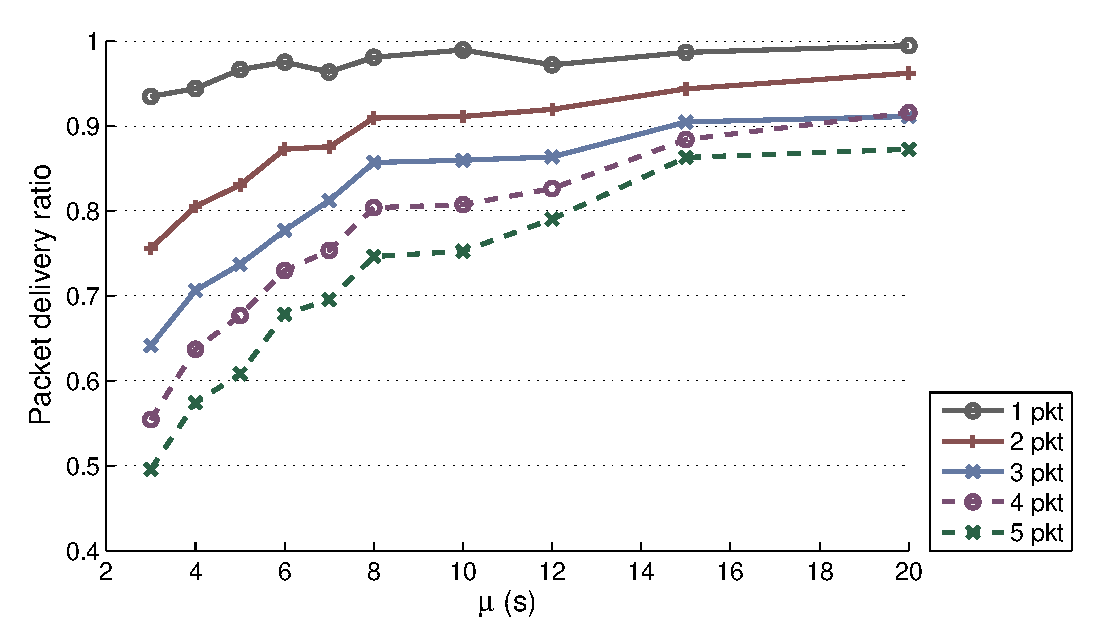
\includegraphics[width=\textwidth] {../../sw/pc/matlab/simulation-result/retrans-count-pdr-20min-pdr1.eps}
        \caption{}
    \end{subfigure}
    \caption[EDR and PDR with different transmission redundancy, $PDR_0 = 1$]{Simulation results showing EDR(a) and PDR(b) with different number of retransmissions per event, at $PDR_0 = 1$}\label{fig:retrans-lambda-1}
\end{figure}

When the events are dense, i.e. shorter $\mu$. Having multiple transmissions do not improve $EDR$, because the number of packets is multiplied, so does the chance of collision. When the events are sparse, i.e. longer $\mu$, the advantage of having multiple transmissions becomes significant, especially with low $PDR_0$. This is more likely to be the case in real settings: sparse events, and some sensors have low $PDR_0$ because of long range or poor link. 

We know that in computer networks, having packets fit into timeslots which are synchronous across senders can reduce collision and improve throughput \cite{Roberts1975}. In our design, packet transmission are synchronized to AC cycles. However, they are not fully synchronized as each timeslot takes 4 AC cycles. Here, through simulation, we evaluate the difference in $EDR$ and $PDR$ with fully asynchronous, 1-cycle-synchronous and 4-cycle-synchronous (fully slotted) systems. 

The result in Fig.\ref{fig:edr-pdr-slotting} shows that synchronizing packets to AC cycles have slight improvement in term of $EDR$ and $PDR$ compared to the case of completely asynchronous. On the other hand, having the packets fully slotted improves the delivery ratios much, compared to the other two cases. Currently, we can synchronize to one cycle by the zero-crossing circuit. We can not currently employ the fully-slotted scheme unless we add other hardware capabilities. Another way is to reduce packet length to less than one AC cycle, which means also raising transmitter power in order to get the same $PDR_0$. 

\begin{figure}[p]
    \centering
    \begin{subfigure}[t]{0.8\textwidth}
        \centering
        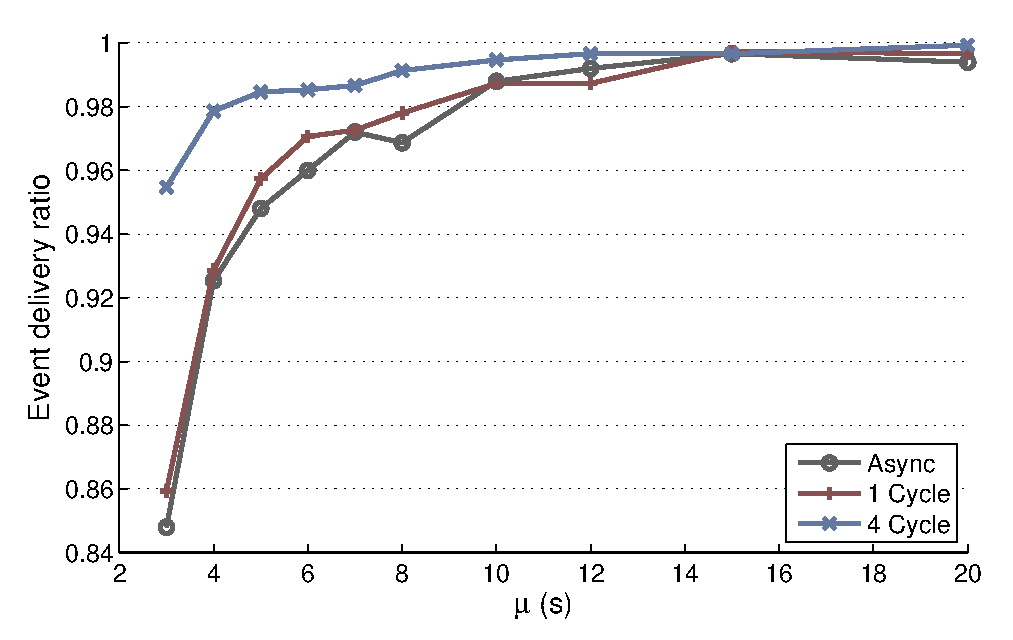
\includegraphics[width=\textwidth] {../../sw/pc/matlab/simulation-result/slotting-edr-250evt.eps}
        \caption{}
    \end{subfigure} 
    \\
    \begin{subfigure}[t]{0.8\textwidth}
        \centering
        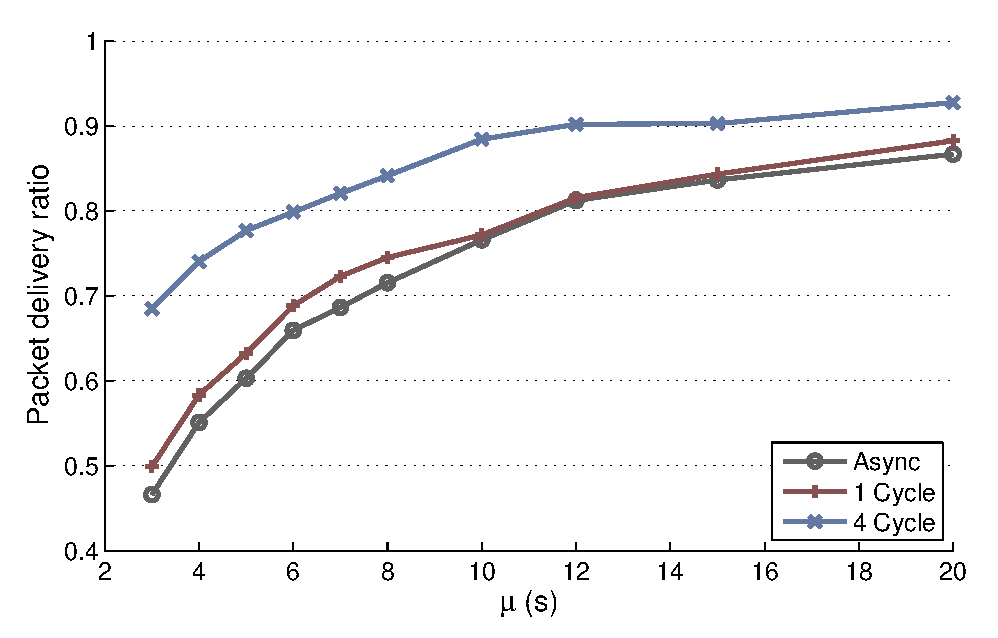
\includegraphics[width=\textwidth] {../../sw/pc/matlab/simulation-result/slotting-pdr-250evt.eps}
        \caption{}
    \end{subfigure}
    \caption[EDR and PDR with different timeslot alignment]{Simulation results showing EDR(a) and PDR(b) with different timeslot alignment}\label{fig:edr-pdr-slotting}
\end{figure}

\subsection{Controlled experiments: Two-events collision test and Poisson distribution events}

We setup a small scale testbed so that we can test real hardware with programmatically controllable events through an extra microcontroller which is connected to a computer. The extra microcontroller, which is an mbed\footnote{http://mbed.org/}, is connected to each sensor with a wire. It toggles the wire to indicate events. The mbed is also connected to the computer with a USB emulated serial port. Therefore, a perl script running on the computer can issue events to the sensors via the mbed. 

The sensors run a slightly modified version of firmware, which enables them to receive events from the digital input pin, instead of using the AC current step changes. Nevertheless, the AC current step change algorithms are still running, in order to emulate the timing of event detection as accurate as possible. The RF transmission code is unmodified. The sensors are plugged into AC sockets and powered with AC, so that the zero-crossing function is also working in the same way as real deployment. 

Firstly, we conduct a event collision test. Since all 5 transmissions of a single event can take up to 2.2s, any two events that happen within 2.2s on two different sensors are considered collided events. Note that two events that happen within 2.2 on a single sensor are not collided, because any pending retransmissions of the first event (flash event) are cancelled. 

\begin{figure}[htb]
  \centering
  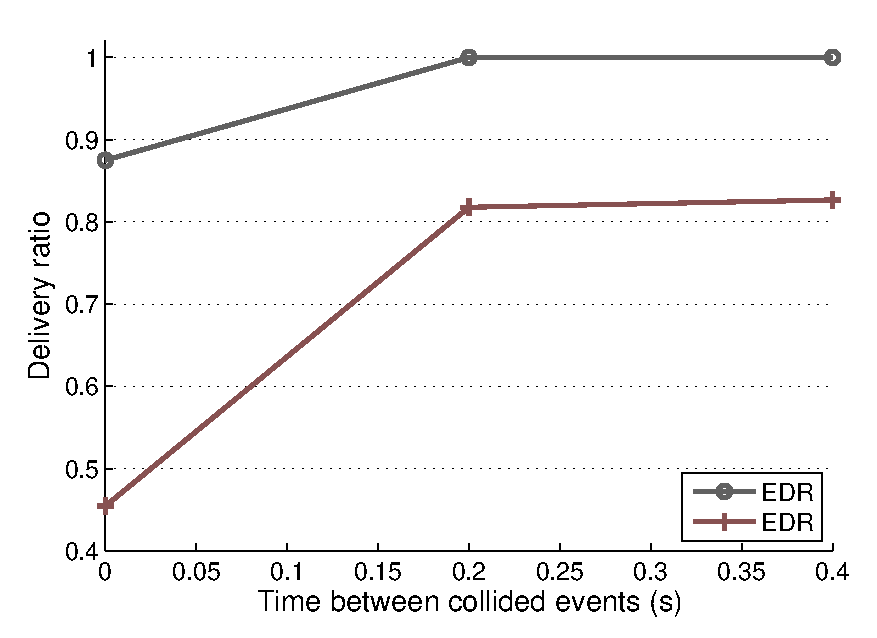
\includegraphics[width=0.7\textwidth]{../../sw/pc/matlab/testbed-result/collision}
  \caption{Two events collision test result}
  \label{fig:collision}
\end{figure}

In this test, we generate collided events with fixed interval, two events at a time for 100 times. Fig.\ref{fig:collision} shows the resulting EDR and PDR. The plots show that when the EDR becomes perfect when the interval between collided events are greater than 0.2s. In real cases, it is unlikely that two events happens at exactly the same time. Even if some appliances are highly correlated in term of their on-off states, such as a DVD player and a TV set, their turn-on time are not strictly aligned. On the other hand, even in the extreme case of two strictly synchronous events, the system can still delivery them at a high probability of 88\%. 

\begin{figure}[htb]
  \centering
  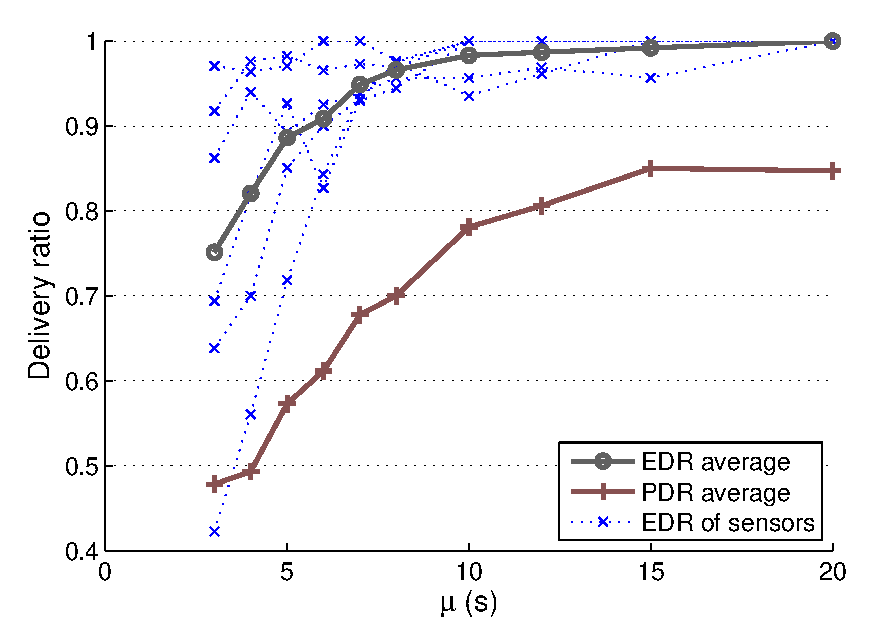
\includegraphics[width=0.7\textwidth]{../../sw/pc/matlab/testbed-result/poisson-5min}
  \caption{Poisson distribution events test}
  \label{fig:poisson-5min}
\end{figure}

Secondly, we use some poisson distribution datasets on the testbed. The datasets are synthesized in the same way as described in the previous section, with $N = 6$, $\mu$ varies from 3 to 20. We limit the length of each dataset to be 300 seconds long. Fig.\ref{fig:poisson-5min} shows the average EDR and PDR, as well as the EDR of separate sensors. We can see that as the event density increases, some sensors are much worse than the others. This is because the transmission power differs among the sensors. The receiver has an automatic gain control (AGC) to tune the receiving signal strength. However, the AGC needs time to settle. When the transmission are too busy, the AGC can not accommodate all sensors. If the events are sparse with longer $\mu$, all sensor nodes have near perfect EDR. Again, even the case with $\mu=20$ is much more denser than a real setting. Appliances are very unlikely to be turned on and off within 20 seconds. 

\subsection{Evaluation in real settings}

In this section, we provide the statistics of the sensor network with a dataset collected in a real setting. We have 21 sensors deployed in our lab, named \#1 through \#22, and \#10 is not deployed. \#16 is deployed, but there is no event during the time window of this dataset. Details about the deployment are discussed in Chapter \ref{chap5}.

The dataset we used for the statistics contains data collected in 18 days. Note that in the real settings, lost packets and lost events are estimated by analyzing the sequence number. This is accurate unless there are more than 16 successive packet loss, which is very rare. Fig.\ref{real-edr-pdr} shows the EDR and PDR of each sensor. We can see that  all sensors achieve almost perfect EDR, except for \#1. Detailed data are shown in Table \ref{tab:recvstat}.

\begin{figure}[htb]
  \centering
  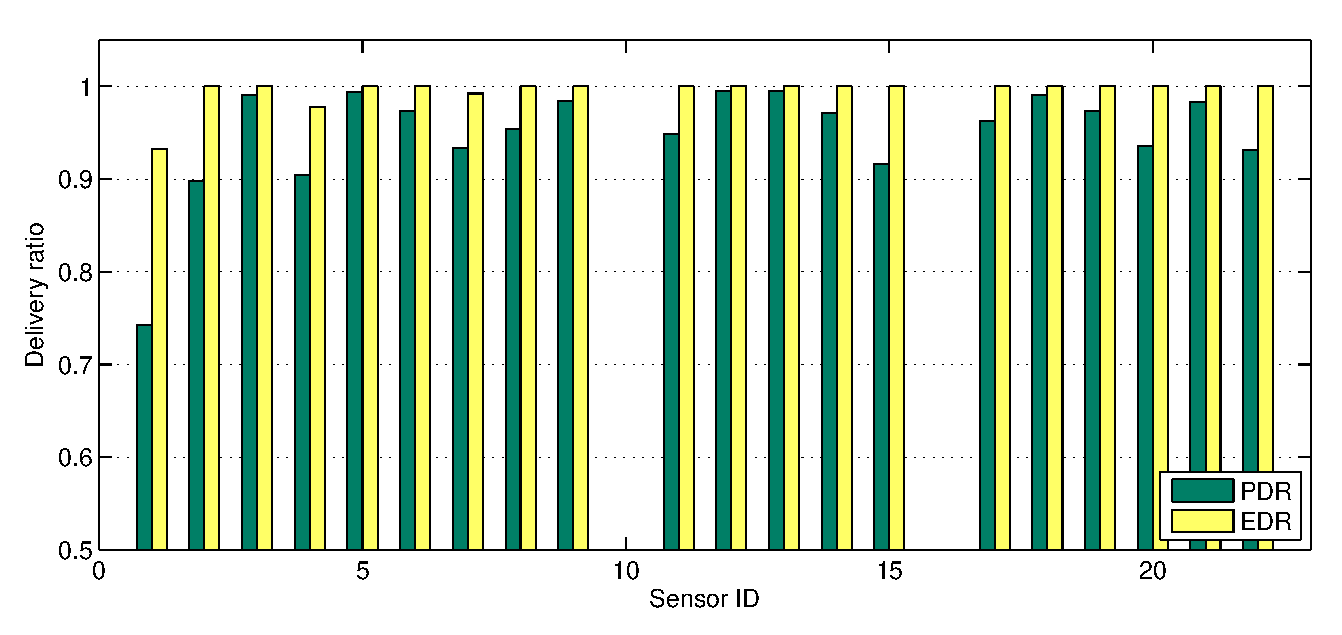
\includegraphics[width=\textwidth]{../../sw/pc/matlab/testbed-result/real}
  \caption{EDR and PDR in a real setting}
  \label{fig:real-edr-pdr}
\end{figure}

\begin{table}
  \centering
  \begin{tabular}{lcccc}
  \hline
  ID & RX Packets & TX packets & RX Events & TX Events \\
  \hline
1&      308     &    415    &      83     &     89\\
  2&       247    &     275   &       64    &      64\\
  3&       628    &     634   &      137    &     137\\
  4&       208    &     230   &       44    &      45\\
  5&       331    &     333   &       67    &      67\\
  6&        37    &      38   &        8    &       8\\
  7&     20364    &   21818   &     4534    &    4569\\
  8&       290    &     304   &       69    &      69\\
  9&       307    &     312   &       81    &      81\\
  10&         0   &        0  &         0   &        0\\
  11&       354   &      373   &       81    &      81\\
  12&       216   &      217  &        54    &      54\\
  13&       438   &      440  &        88    &      88\\
  14&       134   &      138  &        30    &      30\\
  15&        55   &       60  &        12    &      12\\
  16&         0   &        0  &         0    &       0\\
  17&       255   &      265  &        54    &      54\\
  18&      1125   &    1135   &      227     &    227\\
  19&       146   &      150  &        30    &      30\\
  20&       452   &     483   &       97     &     97\\
  21&       586   &     596   &      120     &    120\\
  22&       270   &      290  &        58    &      58 \\ 
  \hline
  Total&    26751   &    28506   &     5938    &    5980 \\ 
  \end{tabular}
  \caption{Sensor network delivery statistics in a real setting}
  \label{tab:recvstat}
\end{table}
